\documentclass[12pt,a4paper]{article}
\usepackage[utf8x]{inputenc}
\usepackage{ucs}
\usepackage{amsmath}
\usepackage{amsfonts}
\usepackage{amssymb}
\usepackage{graphicx}
\usepackage{grffile}
\usepackage{float}
\usepackage{multicol}
\usepackage[portuguese]{babel}
\title{MAT2456 - P2-2014}
\author{André Garnier Coutinho}
\setlength{\textwidth}{17cm}
\setlength{\textheight}{24cm}
\addtolength{\topmargin}{-2cm}
\addtolength{\oddsidemargin}{-2cm}

\newcommand{\re}{\mathbb{R}}

\newcommand{\sen}{\mbox{\, sen}\,}

\begin{document}
%%%%%%%%%%%%%%%%%%%%%%%%%%%%%%%%%%%%%%%%%%TURMA A%%%%%%%%%%%%%%%%%%%%%%%%%%%%%%%%%%%%%%%%%%%%%%%
\begin{center}
\textbf{Instituto de Matemática e Estatística da USP\\
MAT2455 - Cálculo Diferencial e Integral IV para Engenharia\\}
\textbf{2a. Prova - 2o. Semestre 2014 - 13/10/2014}
\end{center}

\noindent {\bf Turma A}

\noindent{\bf Questão 1:}
\begin{itemize}
	\item[a)] (1,0 ponto) Seja $ f(x) = \displaystyle\frac{1}{1+2x^3}$. Calcule $f^{(30)}(0)$.
	
	\item[b)] Obtenha uma expressão para a soma da série $\displaystyle\sum_{n=1}^\infty (-1)^n \, 2^n 9 n^2 x^{3n}$ 
	\item[c)] Encontre um valor para a soma do item $b)$, quando $x = \displaystyle\frac{1}{2}$.
\end{itemize}


\noindent{\bf \\ \\Solução:}
\begin{itemize}
    \item[a)] Sabe-se que $ \displaystyle\frac{1}{1-x} = \displaystyle\sum_{n=0}^\infty x^n $, para $|x|<1$ (soma da PG). Sendo assim:
    
    $$\frac{1}{1 + 2x^3} = \sum_{n=0}^\infty (-2 x^3), |-2x^3| < 1$$
    $$ = \sum_{n=0}^\infty (-1)^n  \, 2^n \, x^{3n}, |x| < \frac{1}{\sqrt[3]{2}} $$
    
    
    Sabe-se que para uma série de potencias positivas $ \, \displaystyle\sum_{k=0}^\infty a_k (x-x_0)^k $, $a_k$ é dado pelo coeficiênte de Taylor: $a_k = \displaystyle\frac{f^{(k)}(x_0)}{k!}$.
    
    Como a série encontrada foi expandida em torno de $x_0 = 0$, temos que: $a_{30} = \displaystyle\frac{f^{(30)}(0)}{30!}$, o qual é coeficiente de $x^{30}$. \\
    
    O termo geral da série obtida é dado por $ \bar{a}_n = (-1)^n  \, 2^n \, x^{3n}$.
    
    Para $n=10$, temos $\bar{a}_{10} = 2^{10} x^{30}$, o que significa que o coeficiente de $x^{30}$ na série é $2^{10}$.
    
    Sendo assim, temos: $ \displaystyle\frac{f^{(30)}(0)}{30!} = 2^{10} $
    
    $$ \therefore f^{(30)} = 2^{10} \, 30! $$


    \item[b)] Deseja-se encontrar uma expressão para $\displaystyle\sum_{n=1}^\infty (-1)^n \, 2^n 9 n^2 x^{3n}$.
    
     Pode-se observar que há uma certa semelhança entre os termos gerais desta série e da série do exercicio anterior. Repare que derivando em x, multiplicando por x, derivando mais uma vez e multplicando por x mais uma vez, chegamos na mesma expressão. Sendo assim:
     
     $$\frac{1}{1 + 2x^3} =  \sum_{n=0}^\infty (-1)^n  \, 2^n \, x^{3n}, |x| < \frac{1}{\sqrt[3]{2}} $$
     
     Derivando em x:
     
     $$\frac{-2 \cdot 3 x^2}{(1 + 2x^3)^2} =  \sum_{n=0}^\infty (-1)^n  \, 2^n \, 3 n \, x^{3n-1}, |x| < \frac{1}{\sqrt[3]{2}} $$
     
     $$ \Rightarrow \frac{-6 x^3}{(1 + 2x^3)^2} =  \sum_{n=0}^\infty (-1)^n  \, 2^n \, 3 n \, x^{3n}, |x| < \frac{1}{\sqrt[3]{2}} $$
     
     Derivando mais uma vez:
     
     $$ \frac{-6 [ (3 x^2) (1 + 2x^3)^2 - x^3 \cdot 2 (1 + 2 x^3) 6 x^2 ] }{(1 + 2x^3)^4} =  \sum_{n=0}^\infty (-1)^n  \, 2^n \, 9 n^2 \, x^{3n-1}, |x| < \frac{1}{\sqrt[3]{2}} $$
     
     $$ \frac{-6 [ 3 x^2 - 6 x^5 ] }{(1 + 2x^3)^3} =  \sum_{n=0}^\infty (-1)^n  \, 2^n \, 9 n^2 \, x^{3n-1}, |x| < \frac{1}{\sqrt[3]{2}} $$
     
     $$ \therefore \sum_{n=0}^\infty (-1)^n  \, 2^n \, 9 n^2 \, x^{3n} = \frac{-18 x^3 (1 - 2 x^3)}{(1 + 2 x^3)^3} , |x| < \frac{1}{\sqrt[3]{2}} $$
     
     \item[c)] Como $ x = \frac{1}{2}$ está dentro do intervalo de convergência da série do item $b)$, temos que:
     
     $$  \sum_{n=0}^\infty   \frac{(-1)^n  \, 9 n^2}{4^n} = \frac{-18 \cdot \frac{1}{8} (1 - 2 \cdot \frac{1}{8})}{(1 + 2  \cdot \frac{1}{8})^3} = -\frac{3^3 4}{5^3} = -\frac{108}{125} $$
    

\end{itemize}
\ \

%---------------------------------------QUESTAO 2-----------------------------------------
\newpage

\noindent{\bf Questão 2}
(3,0 pontos) Calcule a integral

$$ \int \int \int_E xz \,dx \,dy \,dz $$

sobre a região $ E = \{ (x,y,z): x^2 + y^2 + z^2 \leq 36 $ e $ z \geq \sqrt{ x^2 + (y-6)^2 }, x \geq 0 \} $ \\

\noindent{\bf Solução:} \\

O sólido descrito pela região $E$ está compreendido na região acima do cone $z = \sqrt{ x^2 + (y-6)^2 } $ e abaixo da esfera $ x^2 + y^2 + z^2 = 36 $.

\begin{figure}[h!]
	\centering
	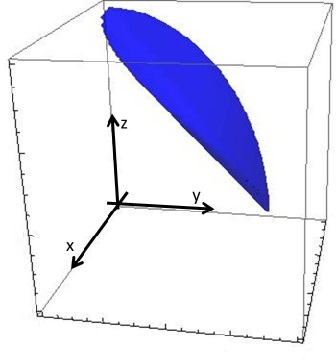
\includegraphics[scale=0.5]{Q2A.jpg}  
	\caption{Região $E$}
	\label{fig:figura4}
\end{figure}

Portanto:

$$ \int \int \int_E xz \,dx \,dy \,dz =  \int \int_R \Big( \int_{ \sqrt{x^2 + (y-6)^2} }^{ \sqrt{36 - x^2 - y^2} } xz \,dz \Big) \,dx \,dy = \int \int_R x \frac{z^2}{2} \Big|_{ \sqrt{x^2 + (y-6)^2} }^{ \sqrt{36 - x^2 - y^2} } \,dx \,dy  $$
$$ = \frac{1}{2} \int \int_R x (-2x^2 - 2y^2 + 12y) \,dx \,dy = - \int \int_R x (x^2 + y^2 - 6y) \,dx \,dy $$ \\

Sendo $R$ a projeção do sólido $E$ no plano $xy$. \\

Realizando a intersecção das 2 superfícies que delimitam o sólido, temos:

$$
\left\{
\begin{array}{lc}
x^2 + y^2 + z^2 = 36\\
z^2 = x^2 + (y-6)^2 \\
\end{array}
\right. \Rightarrow
\left\{
\begin{array}{lc}
2x^2 + y^2 + (y-6)^2 = 36\\
z^2 = x^2 + (y-6)^2 \\
\end{array}
\right.
$$

A projeção no plano $xy$ desta intersecção é dada por:

$$ 2x^2 + y^2 + (y-6)^2 = 36 \Rightarrow 2x^2 + 2y^2 -12y + 36 = 36 \Rightarrow 2x^2 + 2y^2 = 12y $$
$$   \therefore x^2 + y^2 = 6y \Leftrightarrow x^2 + (y-3)^2 = 9 $$

Sendo assim, a região $R$ é dada por:

$$ R = \{ (x,y): x^2 + (y-3)^2  \leq 9 , x \geq 0 \} $$

\begin{figure}[h!]
	\centering
	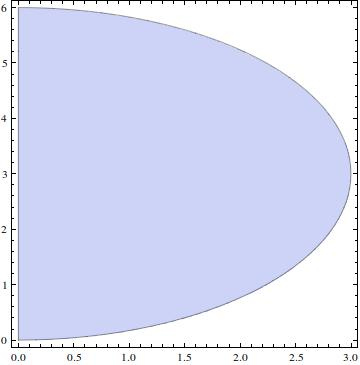
\includegraphics[scale=0.5]{Q2bA.jpg}  
	\caption{Região $R$}
	\label{fig:figura5}
\end{figure}

Realizando uma mudança de coordenadas para coordenadas polares:

$$
\left\{
\begin{array}{lc}
x = \rho \cos \theta\\
y = \rho \sin \theta \\
\end{array}
\right.
$$
$$ | \det J | = \rho $$

Substituindo a mudança na equação da fronteira de $R$:

$$ x^2 + y^2 = 6y \Rightarrow \rho^2 = 6 \rho \sin \theta \Rightarrow \rho = 6 \sin \theta $$

Sendo assim, a região $R$ pode ser escrita em coordenadas polares da seguinte maneira:

$$ 0 \leq \rho \leq  \ 6 \sin \theta $$
$$ 0 \leq \theta \leq \frac{\pi}{2} $$

Aplicando a mudança na integral, temos:


$$- \int \int_R x (x^2 + y^2 - 6y) \,dx \,dy  = - \int_0^{\frac{\pi}{2}} \int_0^{6 \sin \theta} \rho \cos \theta ( \rho^2 - 6 \rho \sin \theta ) \rho \,d\rho
 \,d\theta $$
 $$ =  - \int_0^{\frac{\pi}{2}} \int_0^{6 \sin \theta} ( \rho^4 \cos \theta - 6 \rho^3 \sin \theta \cos \theta ) \,d\rho
 \,d\theta = - \int_0^{\frac{\pi}{2}}  \Big( \frac{\rho^5}{5} \Big|_0^{6 \sin \theta} \cos \theta - 6 \frac{\rho^4}{4} \Big|_0^{6 \sin \theta} \sin \theta \cos \theta \Big) 
 \,d\theta  $$
 $$ = 6^5 \Big( \frac{1}{4} - \frac{1}{5} \Big) \int_0^{\frac{\pi}{2}} \sin^5 \theta \cos \theta \,d\theta  $$
 
 Realizando a seguinte mudança de variáveis: $u = \sin \theta \Rightarrow du = \cos \theta \,d\theta $, temos:
 
$$ = \frac{6^5}{20} \int_0^1 u^5 \,du = \frac{6^5}{20} \frac{u^6}{6} \Big|_0^1 = \frac{6^4}{20} = \frac{324}{5}$$

\newpage
\noindent{\bf Questão 3: }
(3,0 pontos) Calcule a massa do sólido dado por:
$$u^2+v^2+w^2 \geq 1$$
$$u \geq \sqrt{3v^2+3w^2}$$
$$u\leq 4$$

tal que $w\geq 0$ e com densidade $\displaystyle{\delta(u,v,w)=\frac{1}{\sqrt{u^2+v^2+w^2}}}$\\
\noindent{\bf Solução:}
\\

O sólido está compreendido na região interna ao cone, exterior à esfera e inferior ao plano, conforme visto na figura abaixo:

\begin{figure}[h!]
	\centering
	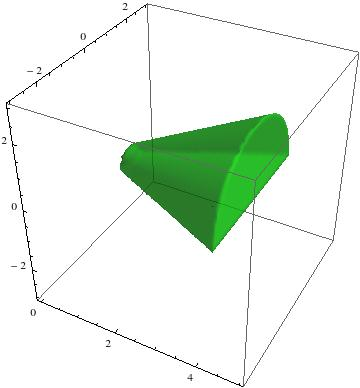
\includegraphics[scale=0.5]{Q3A.jpg}  
	\caption{Esboço do sólido}
	\label{fig:figura6}
\end{figure}

A massa do sólido pode ser calculada por:
$$ Massa = \int\!\!\int\!\!\int_{D_{u,v,w}} \delta(u,v,w)\,du\,dv\,dw $$

Faz-se a mudança para coordenadas esféricas e as regiões ficam descritas por:
$$\left\{\begin{array}{lc}
u=\rho \cdot \cos{\phi}\\
v=\rho \cdot \sen{\theta}\cdot \sen{\phi}\\
w=\rho \cdot \cos{\theta}\cdot \sen{\phi} \\
|J(\rho,\theta,\phi)|=\rho^2 \cdot \sen{\phi}
\end{array}\right.
$$
\\
Assim o domínio de integração em coordenadas esféricas fica:\\
$$D_{\rho,\theta,\phi}= \left\{-\frac{\pi}{2} \leq \theta \leq \frac{\pi}{2}\, \,\, , \,\, 1 \leq \rho \leq \frac{4}{\cos{\phi}}\, \, \mbox{  e  } 
\,\,0 \leq \phi \leq \frac{\pi}{6}\right\}$$

Logo:
\begin{eqnarray*}
\mbox{Massa} &=& \int\!\!\int\!\!\int_{D_{u,v,w}} \delta(u,v,w)\,du\,dv\,dw = \int\!\!\int\!\!\int_{D_{\rho,\theta,\phi}} \delta(\rho,\theta,\phi)\cdot |J(\rho,\theta,\phi)|\,d\rho\,d\theta\,d\phi\\
&=& \int_{-\frac{\pi}{2}}^{\frac{\pi}{2}}\!\!\!\int_{0}^{\frac{\pi}{6}}\!\!\!\int_1^{\frac{4}{\cos{\phi}}}\frac{\rho^2\sen{\phi}}{\rho}\,d\rho\,d\phi\,d\theta\\
&=& \frac{\pi}{2} \int_0^{\frac{\pi}{6}} \rho^2\sen{\phi}\Big|_1^{\frac{4}{\cos{\phi}}}\,d\phi\\
&=& \frac{\pi}{2} \int_0^{\frac{\pi}{6}} 16\frac{\sen{\phi}}{\cos^2{\phi}}-\sen{\phi}\,d\phi\\
&=& 8\pi \frac{1}{\cos{\phi}}\Big|_0^{\frac{\pi}{6}} + \frac{\pi}{2}\cos{\phi}\Big|_0^{\frac{\pi}{6}}\\
&=& 8\pi\left(\frac{2}{\sqrt{3}}-1\right) + \frac{\pi}{2}\left(\frac{\sqrt{3}}{2}-1\right)\\
M &=& \frac{67\pi \sqrt{3}-102 \pi}{12}
\end{eqnarray*}



\newpage
\begin{center}
\textbf{Instituto de Matemática e Estatística da USP\\
MAT2455 - Cálculo Diferencial e Integral III para Engenharia\\}
\textbf{1a. Prova - 1o. Semestre 2014 - 01/04/2010}
\end{center}

\noindent {\bf Turma B}

\noindent{\bf Questão 1:}(4,0 pontos)
\begin{itemize}
	\item[(a)] Calcule $ \displaystyle{ \int_{0}^{3}  \int_{\ln{(x+1)}}^{\ln{4}} \cos{(y-e^y)}\,dy\, dx } $.
	
	\item[(b)] Calcule $\displaystyle{\int\!\!\!\int_R \frac{(y-2x)^8}{(y+x)^5}\,dx\,dy}$, onde $R$ é a região limitada pelas retas $y=2x$, $y=2+2x$,$y=2-x$ e $y=3-x$
	
\end{itemize}


\noindent{\bf \\ \\Solução:}
\begin{itemize}
    \item[(a)] Esboçando o domínio de integração, teremos:
    \\
    

\begin{figure}[h!]
	\centering
	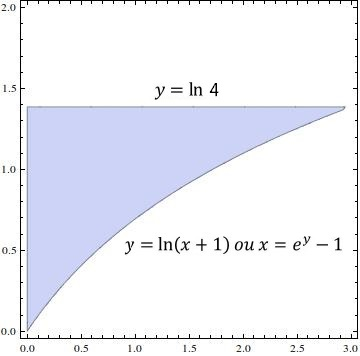
\includegraphics[scale=0.5]{Q1aB.jpg}  
	\caption{Domínio de integração}
	\label{fig:figura7}
\end{figure}

Não é possível encontrar uma primitiva em $y$ para a função do integrando. Para calcular a integral é necessário inverter a ordem de integração. Baseado na imagem acima, o domínio pode ser expresso, também, por:
$$D(x,y)=\{(x,y)\in\re^2 | 0\leq x \leq e^y-1\,\, \mbox{,}\,\,0\leq y \leq \ln{4}\}$$

A integral será calculada por:
\begin{eqnarray*}
&=&\int_0^{\ln{4}}\!\!\!\int_0^{e^y-1}\cos{(y-e^y)}\,dx\,dy\\
&=&\int_0^{\ln{4}} (e^y-1)\cos{(y-e^y)}\,dy\\
&=&-\sin{(y-e^y)}\Big|_0^{\ln{4}}\\
&=&-\sin{(\ln{4}-4)}+\sin{(-1)}
\end{eqnarray*}


    \item[(b)] O domínio de integração é exibido abaixo

\begin{figure}[h!]
	\centering
	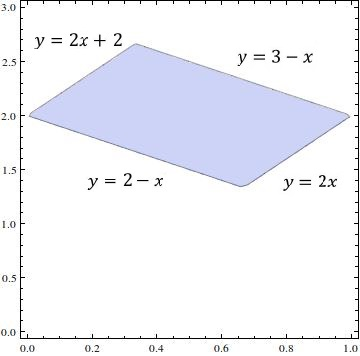
\includegraphics[scale=0.5]{Q1bB.jpg}  
	\caption{Domínio de integração}
	\label{fig:figura8}
\end{figure}
    
Faz-se a seguinte mudança de coordenadas:
    $$\left\{
	\begin{array}{lr}
	u = y-2x\\
	v = y+x
	\end{array}
	\right. 
	$$
    
O jacobiano da transformação é dado por:

$$
\frac{\partial(x,y)}{\partial(u,v)}=
\left|
\begin{array}{cc}
-\frac{1}{3} & \frac{1}{3} \\
\frac{1}{3} & \frac{2}{3}\\
\end{array}
\right|
=-\frac{1}{3} \Rightarrow |J|=\frac{1}{3}\\
$$    

O domínio de integração é exibido abaixo

\begin{figure}[h!]
	\centering
	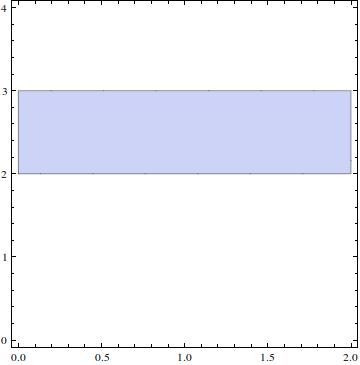
\includegraphics[scale=0.5]{Q1b2B.jpg}  
	\caption{Domínio de integração após mudança}
	\label{fig:figura9}
\end{figure}

E passa a ser dado por:

$$D(u,v)=\{(u,v)\in \re^2|0\leq u \leq 2\,\,\mbox{,}\,\,2 \leq v \leq 3 \}$$

A integral a ser calculada passa a ser:

\begin{eqnarray*}
&=&\int_0^2\!\!\!\int_2^3 \frac{1}{3}\frac{u^8}{v^5}\,dv\,du\\
&=&\frac{1}{3} \int_0^2\!\!\!\int_2^3 u^8.v^{-5}\,dv\,du\\
&=& -\frac{1}{12}\int_0^2 v^{-4}\Big|_2^3 u^8\,du\\
&=& \frac{65}{15552}\frac{u^9}{9}\Big|_0^2\\
&=& \frac{520}{2187}
\end{eqnarray*}
    

\end{itemize}
\ \

%---------------------------------------QUESTAO 2-----------------------------------------
\newpage

\noindent{\bf Questão 2}
(3,0 pontos) Calcule a integral

$$ \int \int \int_E xz \,dx \,dy \,dz $$

sobre a região $ E = \{ (x,y,z): x^2 + y^2 + z^2 \leq 16 $ e $ z \geq \sqrt{ x^2 + (y-4)^2 }, x \geq 0 \} $ \\

\noindent{\bf Solução:} \\

O sólido descrito pela região $E$ está compreendido na região acima do cone $z = \sqrt{ x^2 + (y-4)^2 } $ e abaixo da esfera $ x^2 + y^2 + z^2 = 16 $.

\begin{figure}[h!]
	\centering
	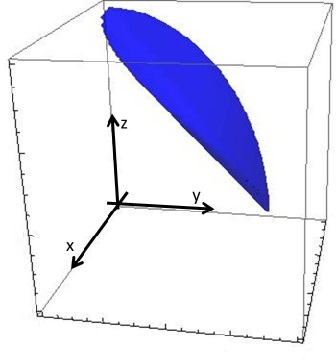
\includegraphics[scale=0.5]{Q2A.jpg}  
	\caption{Região $E$}
	\label{fig:figura10}
\end{figure}

Portanto:

$$ \int \int \int_E xz \,dx \,dy \,dz =  \int \int_R \Big( \int_{ \sqrt{x^2 + (y-4)^2} }^{ \sqrt{16 - x^2 - y^2} } xz \,dz \Big) \,dx \,dy = \int \int_R x \frac{z^2}{2} \Big|_{ \sqrt{x^2 + (y-4)^2} }^{ \sqrt{16 - x^2 - y^2} } \,dx \,dy  $$
$$ = \frac{1}{2} \int \int_R x (-2x^2 - 2y^2 + 8y) \,dx \,dy = - \int \int_R x (x^2 + y^2 - 4y) \,dx \,dy $$ \\

Sendo $R$ a projeção do sólido $E$ no plano $xy$. \\

Realizando a intersecção das 2 superfícies que delimitam o sólido, temos:

$$
\left\{
\begin{array}{lc}
x^2 + y^2 + z^2 = 16\\
z^2 = x^2 + (y-4)^2 \\
\end{array}
\right. \Rightarrow
\left\{
\begin{array}{lc}
2x^2 + y^2 + (y-4)^2 = 16\\
z^2 = x^2 + (y-4)^2 \\
\end{array}
\right.
$$

A projeção no plano $xy$ desta intersecção é dada por:

$$ 2x^2 + y^2 + (y-4)^2 = 16 \Rightarrow 2x^2 + 2y^2 -8y + 16 = 16 \Rightarrow 2x^2 + 2y^2 = 8y $$
$$   \therefore x^2 + y^2 = 4y \Leftrightarrow x^2 + (y-2)^2 = 4 $$

Sendo assim, a região $R$ é dada por:

$$ R = \{ (x,y): x^2 + (y-2)^2  \leq 4 , x \geq 0 \} $$

\begin{figure}[h!]
	\centering
	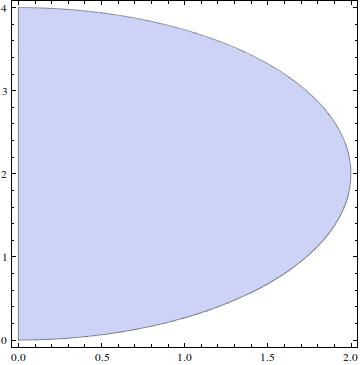
\includegraphics[scale=0.5]{Q2bB.jpg}  
	\caption{Região $R$}
	\label{fig:figura11}
\end{figure}

Realizando uma mudança de coordenadas para coordenadas polares:

$$
\left\{
\begin{array}{lc}
x = \rho \cos \theta\\
y = \rho \sin \theta \\
\end{array}
\right.
$$
$$ | \det J | = \rho $$

Substituindo a mudança na equação da fronteira de $R$:

$$ x^2 + y^2 = 4y \Rightarrow \rho^2 = 4 \rho \sin \theta \Rightarrow \rho = 4 \sin \theta $$

Sendo assim, a região $R$ pode ser escrita em coordenadas polares da seguinte maneira:

$$ 0 \leq \rho \leq  \ 4 \sin \theta $$
$$ 0 \leq \theta \leq \frac{\pi}{2} $$

Aplicando a mudança na integral, temos:


$$- \int \int_R x (x^2 + y^2 - 4y) \,dx \,dy  = - \int_0^{\frac{\pi}{2}} \int_0^{4 \sin \theta} \rho \cos \theta ( \rho^2 - 4 \rho \sin \theta ) \rho \,d\rho
 \,d\theta $$
 $$ =  - \int_0^{\frac{\pi}{2}} \int_0^{4 \sin \theta} ( \rho^4 \cos \theta - 4 \rho^3 \sin \theta \cos \theta ) \,d\rho
 \,d\theta = - \int_0^{\frac{\pi}{2}}  \Big( \frac{\rho^5}{5} \Big|_0^{4 \sin \theta} \cos \theta - 4 \frac{\rho^4}{4} \Big|_0^{4 \sin \theta} \sin \theta \cos \theta \Big) 
 \,d\theta  $$
 $$ = 4^5 \Big( \frac{1}{4} - \frac{1}{5} \Big) \int_0^{\frac{\pi}{2}} \sin^5 \theta \cos \theta \,d\theta  $$
 
 Realizando a seguinte mudança de variáveis: $u = \sin \theta \Rightarrow du = \cos \theta \,d\theta $, temos:
 
$$ = \frac{4^5}{20} \int_0^1 u^5 \,du = \frac{4^5}{20} \frac{u^6}{6} \Big|_0^1 = \frac{4^5}{20 \cdot 6} = \frac{256}{30}$$

\newpage
\noindent{\bf Questão 3: }
(3,0 pontos) Calcule a massa do sólido dado por:
$$u^2+v^2+w^2 \geq 1$$
$$u \geq \sqrt{3v^2+3w^2}$$
$$u\leq 6$$

tal que $w\geq 0$ e com densidade $\displaystyle{\delta(u,v,w)=\frac{1}{\sqrt{u^2+v^2+w^2}}}$\\
\noindent{\bf Solução:}
\\

O sólido está compreendido na região interna ao cone, exterior à esfera e inferior ao plano, conforme visto na figura abaixo:

\begin{figure}[h!]
	\centering
	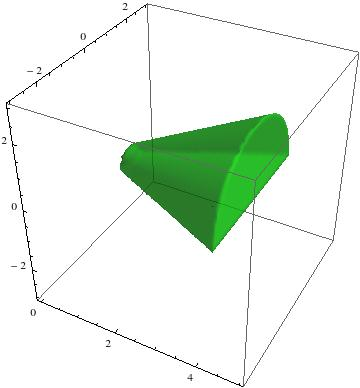
\includegraphics[scale=0.5]{Q3A.jpg}  
	\caption{Esboço do sólido}
	\label{fig:figura12}
\end{figure}

A massa do sólido pode ser calculada por:
$$ Massa = \int\!\!\int\!\!\int_{D_{u,v,w}} \delta(u,v,w)\,du\,dv\,dw $$

Faz-se a mudança para coordenadas esféricas e as regiões ficam descritas por:
$$\left\{\begin{array}{lc}
u=\rho \cdot \cos{\phi}\\
v=\rho \cdot \sen{\theta}\cdot \sen{\phi}\\
w=\rho \cdot \cos{\theta}\cdot \sen{\phi} \\
|J(\rho,\theta,\phi)|=\rho^2 \cdot \sen{\phi}
\end{array}\right.
$$
\\
Assim o domínio de integração em coordenadas esféricas fica:\\
$$D_{\rho,\theta,\phi}= \left\{- \frac{\pi}{2}  \leq \theta \leq \frac{\pi}{2} \, \,\, , \,\, 1 \leq \rho \leq \frac{6}{\cos{\phi}}\, \, \mbox{  e  } 
\,\,0 \leq \phi \leq \frac{\pi}{6}\right\}$$

Logo:
\begin{eqnarray*}
\mbox{Massa} &=& \int\!\!\int\!\!\int_{D_{u,v,w}} \delta(u,v,w)\,du\,dv\,dw = \int\!\!\int\!\!\int_{D_{\rho,\theta,\phi}} \delta(\rho,\theta,\phi)\cdot |J(\rho,\theta,\phi)|\,d\rho\,d\theta\,d\phi\\
&=& \int_{-\frac{\pi}{2}}^{\frac{\pi}{2}}\!\!\!\int_{0}^{\frac{\pi}{6}}\!\!\!\int_1^{\frac{6}{\cos{\phi}}}\frac{\rho^2\sen{\phi}}{\rho}\,d\rho\,d\phi\,d\theta\\
&=& \frac{\pi}{2} \int_0^{\frac{\pi}{6}} \rho^2\sen{\phi}\Big|_1^{\frac{6}{\cos{\phi}}}\,d\phi\\
&=& \frac{\pi}{2} \int_0^{\frac{\pi}{6}} 36\frac{\sen{\phi}}{\cos^2{\phi}}-\sen{\phi}\,d\phi\\
&=& 18\pi \frac{1}{\cos{\phi}}\Big|_0^{\frac{\pi}{6}} + \frac{\pi}{2}\cos{\phi}\Big|_0^{\frac{\pi}{6}}\\
&=& 18\pi\left(\frac{2}{\sqrt{3}}-1\right) + \frac{\pi}{2}\left(\frac{\sqrt{3}}{2}-1\right)\\
M &=& \frac{49 \pi \sqrt{3} - 74 \pi}{4}
\end{eqnarray*}

\end{document} 
